%%%%%%%%%%%%%%%%%%%%%%%%%%%%%%%%%%%%%%%%%%%%%%%%%%%%%%%%
%%%%%%%%%%%%%%%%%%%%%%%%%%%%%%%%%%%%%%%%%%%%%%%%%%%%%%%%
\section{Results}
\label{sec:results}
%%%%%%%%%%%%%%%%%%%%%%%%%%%%%%%%%%%%%%%%%%%%%%%%%%%%%%%%
%%%%%%%%%%%%%%%%%%%%%%%%%%%%%%%%%%%%%%%%%%%%%%%%%%%%%%%%
%
%%%%%%%%%%%%%%%%%%%%%%%%%%%%%%%%%%%%%%%%%%%%%%%%%%%%%%%%
\subsection{Mapping Performance}
\label{ssec:mapping_performance}
%%%%%%%%%%%%%%%%%%%%%%%%%%%%%%%%%%%%%%%%%%%%%%%%%%%%%%%%
%
We produced FIMs for the entire BLE domain within the 49 HUC8 area across several states in the south central US. 
The forecasted FIMs using the discharges for the 1\% (100 year) and 0.2\% (500 year) recurrence flows directly from HEC-RAS were used to avoid noise and errors from hydrological processes.
We computed the statistics (CSI, POD, and FAR) for both 100 and 500 year events for Mannings N set to 0.06 and 0.12. 
The distribution of these statistics can be examined in Figure \ref{fig:violin_plot} as violin plots.
Each half of a violin plot represents the kernel density estimation (KDE) for a given model (FR, MS, GMS), given Manning's N value (0.06, 0.12), and given recurrence interval (1\%, 0.2\%), and performance metric (CSI, POD, FAR).
We also denote trend lines for each metric and Manning's n setting as well as their respective slope estimate and one-tailed p-value denoting the level of significance of the trend.

Aggregating the metrics in the method above treats each HUC8 as it's own unit and does little to consider the size differences of the HUCs. 
In an opposing aggregation method, we illustrate in Table \ref{tab:aggregate_metrics} the sum of all the TPs, FPs, and FNs to recompute CSI, POD, and FAR across the entire domain. 
%
\begin{table}[h!]
\caption{Primary metrics, TPs, FPs, and FNs, aggregated for BLE domain to recompute CSI, POD, and FAR.}
\label{tab:aggregate_metrics}
\centering
%\begin{tabular}{|p{2cm}|p{2cm}|p{2cm}|p{2cm}|}
\begin{tabular}{|c|c||c|c|c|c|c|c|}
\hline
\multirow{2}{*}{Metric} & \multirow{2}{*}{Manning's N} & \multicolumn{2}{|c|}{FR} & \multicolumn{2}{|c|}{MS} & \multicolumn{2}{|c|}{GMS} \\
\cline{3-8}
  &  & 100yr & 500yr & 100yr & 500yr & 100yr & 500yr \\
\hline
\multirow{2}{*}{CSI} & 0.06 & 0.5576 & 0.5839 & 0.5717 & 0.5990 & 0.5796 & 0.6075 \\
\cline{2-8}
  & 0.12 & 0.5915 & 0.6149 & 0.6054 & 0.6288 & 0.6182 & 0.6435 \\
\hline
\multirow{2}{*}{POD} & 0.06 & 0.6354 & 0.6575 & 0.6524 & 0.6755 & 0.6633 & 0.6863 \\
\cline{2-8}
  & 0.12 & 0.7255 & 0.7446 & 0.7460 & 0.7648 & 0.7606 & 0.7810 \\
\hline
\multirow{2}{*}{FAR} & 0.06 & 0.1800 & 0.1609 & 0.1778 & 0.1589 & 0.1787 & 0.1589 \\
\cline{2-8}
  & 0.12 & 0.2379 & 0.2208 & 0.2374 & 0.2204 & 0.2324 & 0.2148 \\
\hline
\end{tabular}
\end{table}
%
\begin{figure}[h!]
\centering
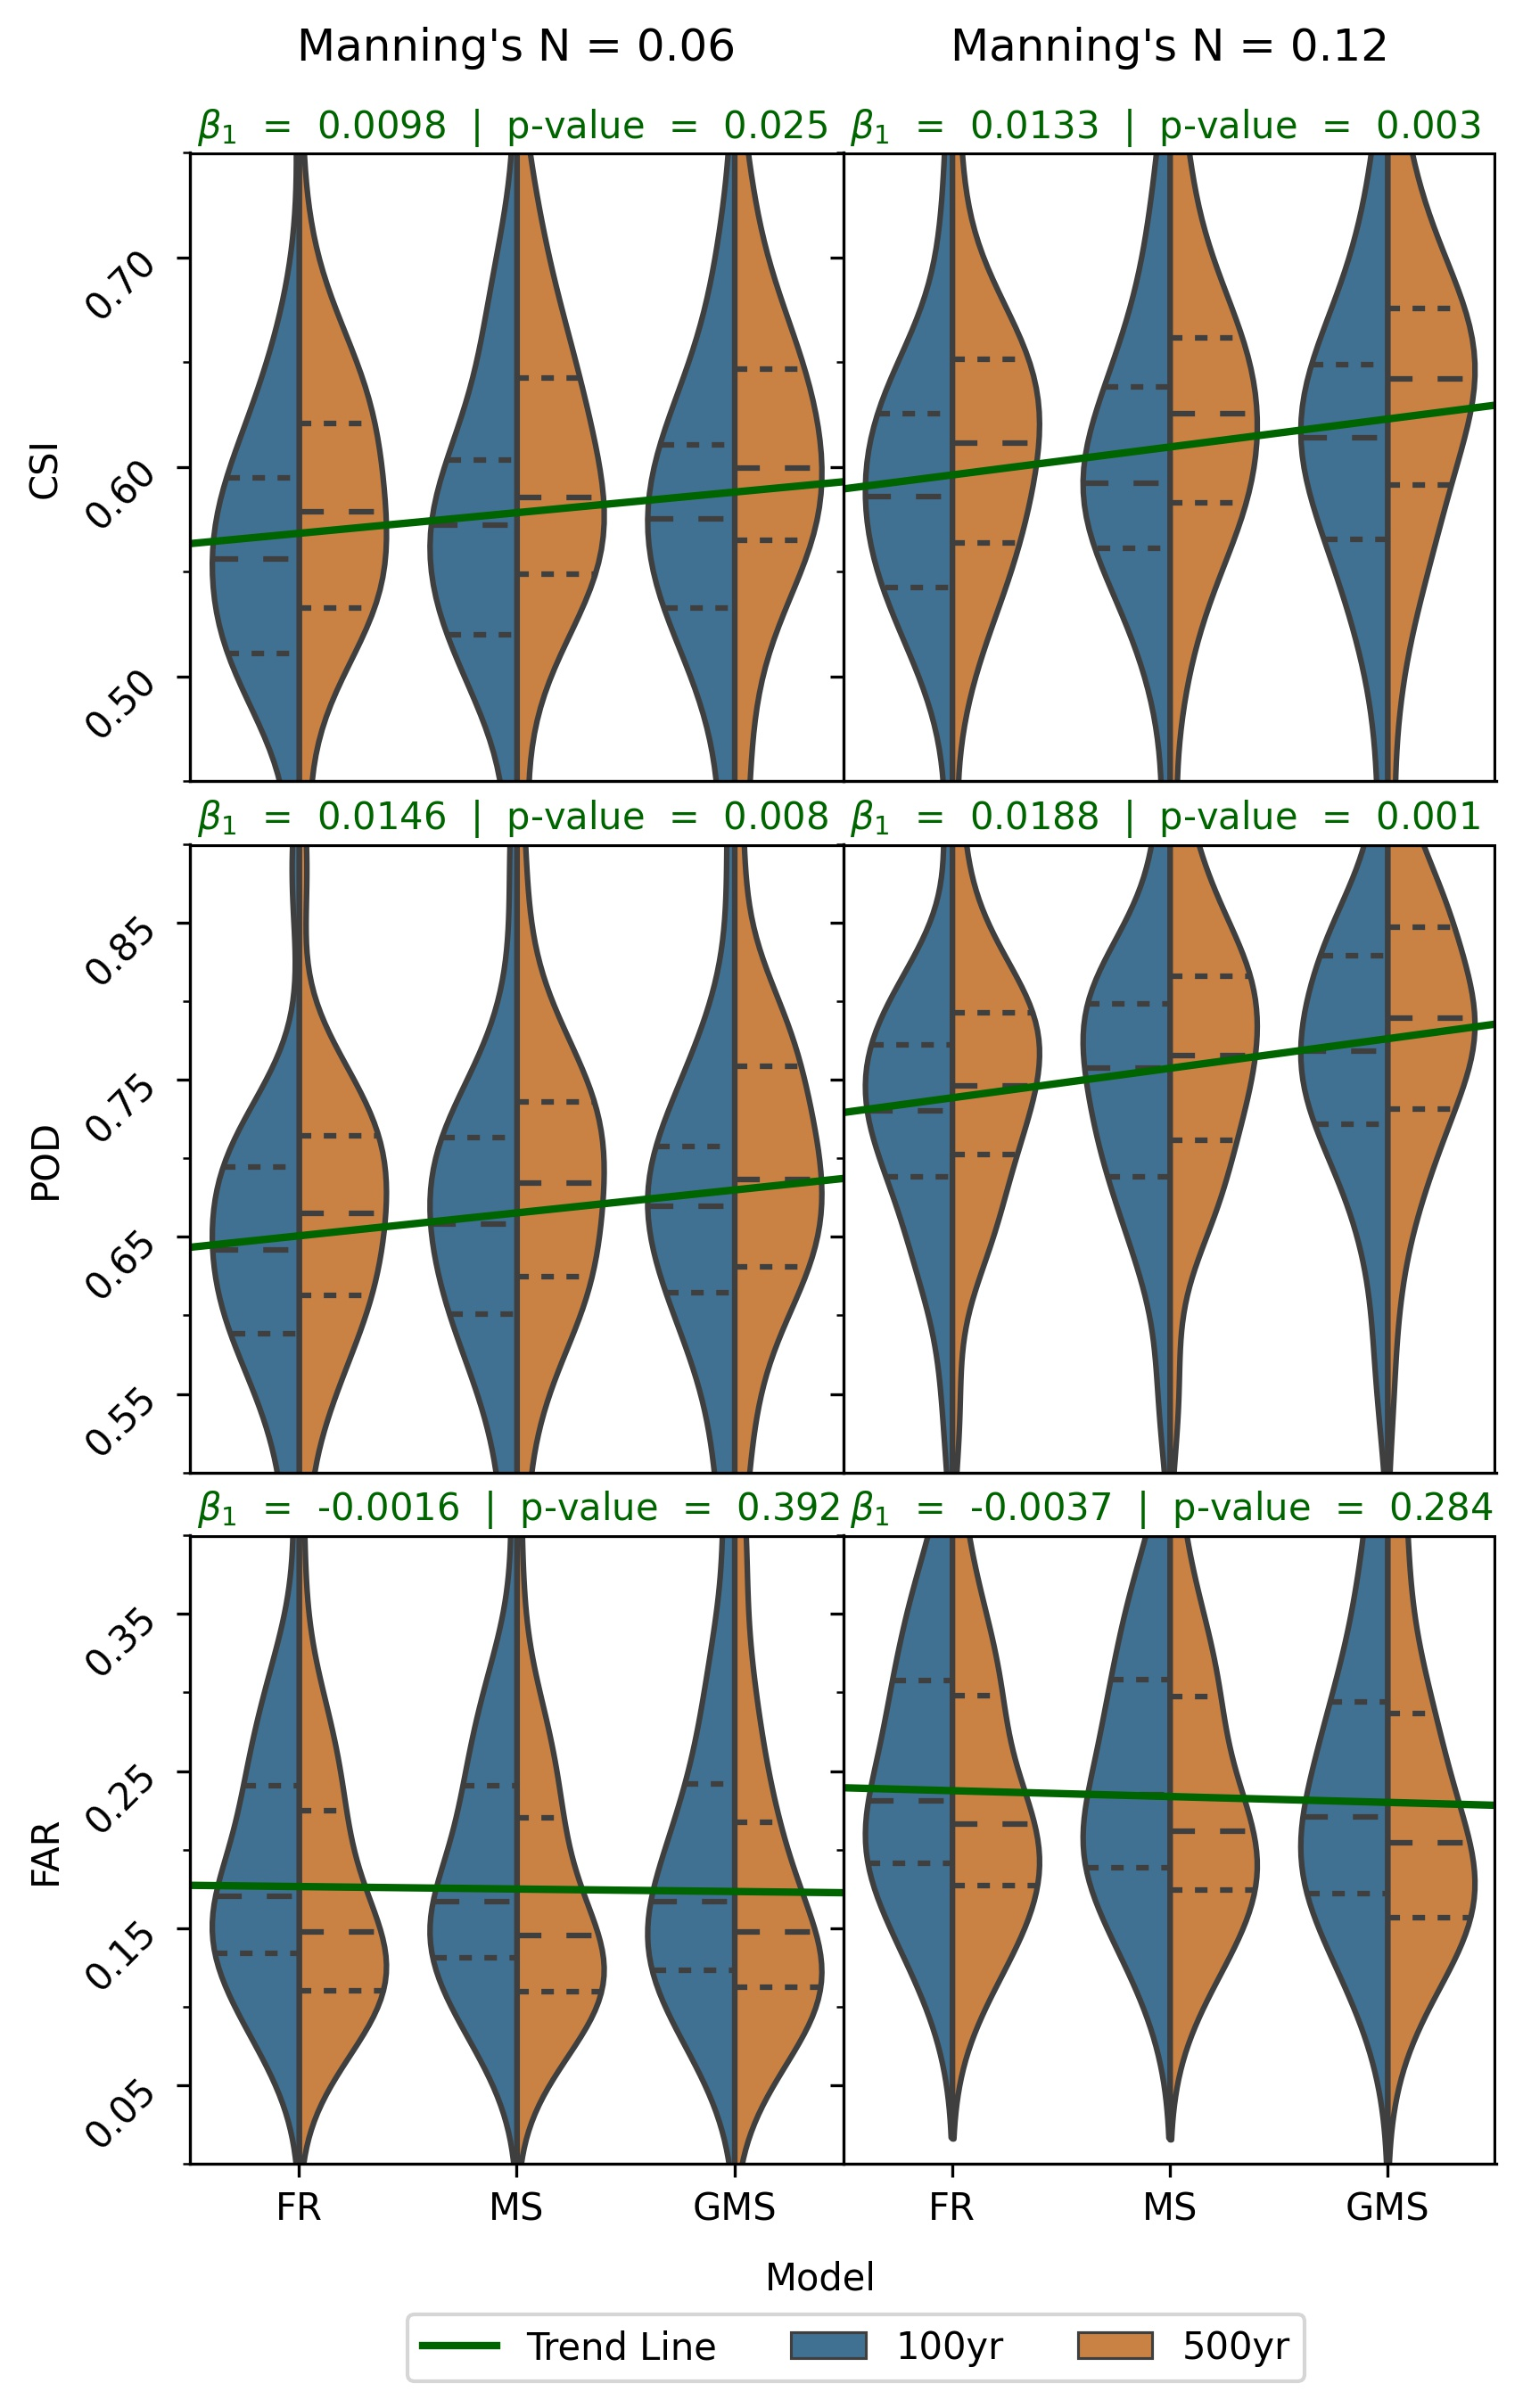
\includegraphics[scale=0.9]{figures/violin_plots.jpg}
\caption{Shows kernel density estimation of the distributions (N = 49) for 1\% (100 year) and 0.2\% (500 year) along with horizontal, dashed lines for the 25th, 50th, and 75th percentiles (in order from bottom to top).
The sub-figures separate the combination of three metrics (CSI, POD, and FAR) for two settings of Manning's N (0.06 and 0.12).
Trend lines for each metric / Mannings combination are shown (N = 294) along with associated slope and p-value of slope testing one-tailed significance.}
\label{fig:violin_plot}
\end{figure}
%
% Interpretation of metrics
From Figure \ref{fig:violin_plot} and Table \ref{tab:aggregate_metrics}, we denote several meaningful trends. 
Using CSI as an overall proxy for skill of the FIM, we note that generally speaking the skill is correlated with a reduction of the stream orders of the processing units used for HAND.
In other words, the more you derive HAND on networks of unit drainage density and mosaic the resulting FIMs, the better those FIMs perform.
While this trend is evident for both sets of Manning's N values, the trend is slightly more significant for the higher value of 0.12.
Other trends related to this figure include the general performance premium for 0.2\% events as opposed to lower 1\% events.
We also note how the higher Manning's N value enhances performance for both of these recurrence intervals across all models.

Dissecting the improvements and trends presented in the previous paragraph comes down mostly to improvement in POD or a reduction in absolute amount of FNs.
POD being the primary driver in skill enhancement is evident across models by comparing the slope of the POD lines with the slope of the FAR lines.
Even though aggregating metrics by HUC8 yields a statistically zero trend, one does see a slight reduction in FAR across models that reduce HAND's maximum stream order.
Additionally, we note that POD is a primary driver in enhancing performance across Manning's N values as well.
This significant improvement comes at a cost of false alarms as the FAR increases significantly across Manning's N values.
%
%%%%%%%%%%%%%%%%%%%%%%%%%%%%%%%%%%%%%%%%%%%%%%%%%%%%%%%%
\subsection{Computational Performance}
\label{ssec:compuational_performance}
%%%%%%%%%%%%%%%%%%%%%%%%%%%%%%%%%%%%%%%%%%%%%%%%%%%%%%%%
%
The NFIE experiments were able to produce HAND for 331 HUC6's in 1.34 CPU years and estimates using work from \citeA{djokic2019arc} put producing HAND at the FR NWM at 0.55 CPU years. 
For our work, we were able to produce HAND at the full NWM resolution in 0.13 CPU years which represents a substantial speed-up compared to previous works.
For the MS resolution an additional, 0.05 CPU years is required on top of this bringing the total to about 0.18 CPU years to produce 2,188 HUC8s that span additional areas not covered in previous HAND versions including Hawaii and Puerto Rico.
GMS which generalizes HAND production to level path scale adds a significant amount of CPU time to the process bringing the estimate total to about 1.17 CPU years \note[Fernando Aristizabal]{Fernando A: Review}.
%
